%Report template by Christian Fischer Pedersen for IT-ONK
%--------------------------------------------------------

%Page layout
%--------------------------------------------------------
\documentclass[a4paper,10pt]{report}
\usepackage{fancyhdr}
\usepackage[left=3cm,right=2cm,top=2cm,bottom=2cm]{geometry}

%Seperated files
%--------------------------------------------------------
\usepackage{subfiles}

%Standard sti at søge efter billeder
\usepackage{graphicx}
\usepackage{float}
\graphicspath{{Figurer/}}

%Speciel skrift for enkelt linje kode
%Udskriver med fonten 'Courier'
%Mere info her: http://tex.stackexchange.com/questions/25249/how-do-i-use-a-particular-font-for-a-small-section-of-text-in-my-document
\newcommand{\code}[1]{{\fontfamily{pcr}\selectfont #1}}

%FixMe pakken viser små kommentarer, hvor der skal rettes
%Brug med følgende: \fxnote{det her skal uddybes!}
%Se liste over alle sixMe's: \listoffixmes
\usepackage[footnote,draft,danish,silent,nomargin]{fixme}

%----------------------------------------------------------
% Følgende er til koder.
% Indsættes mellem \begin{lstlisting} og \end{lstlisting}
% Se eksempel under pakken
%----------------------------------------------------------
\usepackage{listings}
\usepackage{color}
\usepackage{textcomp}
\definecolor{listinggray}{gray}{0.9}
\definecolor{lbcolor}{rgb}{0.9,0.9,0.9}
\renewcommand{\lstlistingname}{Code snippet}
\lstdefinestyle{Code}
{
	title 			= Code snippet,
	keywordstyle	= \bfseries\ttfamily\color[rgb]{0,0,1},
	identifierstyle	= \ttfamily,
	commentstyle	= \color[rgb]{0.133,0.545,0.133},
	stringstyle		= \ttfamily\color[rgb]{0.627,0.126,0.941},
	showstringspaces= false,
	basicstyle		= \small,
	numberstyle		= \footnotesize,
%	numbers			= left, % Tal? Udkommenter hvis ikke
	stepnumber		= 2,
	numbersep		= 6pt,
	tabsize			= 2,
	breaklines		= true,
	prebreak 		= \raisebox{0ex}[0ex][0ex]{\ensuremath{\hookleftarrow}},
	breakatwhitespace= false,
%	aboveskip		= {1.5\baselineskip},
  	columns			= fixed,
  	upquote			= true,
  	extendedchars	= true,
 	backgroundcolor = \color{lbcolor},
	lineskip		= 1pt,
%	xleftmargin		= 17pt,
%	framexleftmargin= 17pt,
	framexrightmargin	= 0pt, %6pt
%	framexbottommargin	= 4pt,
}


%Custom length for caption over lstlisting
%The caption must be 6 pt shorter
\usepackage{calc}
\newlength{\mywidth}
\setlength{\mywidth}{\textwidth-6pt}


% Customized style for the caption
\usepackage{caption}
\DeclareCaptionFont{white}{\color{white}}
\DeclareCaptionFormat{listing}%
{\colorbox[cmyk]{0.43, 0.35, 0.35,0.35}{\parbox{\mywidth}{\hspace{5pt}#1#2#3}}}
\captionsetup[lstlisting]
{
	format			= listing,
	labelfont		= white,
	textfont		= white, 
	singlelinecheck	= false, 
	width			= \mywidth,
	margin			= 0pt, 
	font			= {bf,footnotesize}
}

\lstdefinestyle{Code-C} {language=C, style=Code}
\lstdefinestyle{Code-C++} {language=[Visual]C++, style=Code}
\lstdefinestyle{Code-VHDL} {language=VHDL, style=Code}
\lstdefinestyle{Code-Bash} {language=Bash, style=Code}

%Text typesetting
%--------------------------------------------------------
\usepackage{bookman}                  
\usepackage[T1]{fontenc}              
\usepackage[utf8]{inputenc}         
\usepackage[english]{babel}        
\usepackage[bf,small,raggedright,compact]{titlesec}
\usepackage[parfill]{parskip}
\usepackage{setspace}
\setcounter{secnumdepth}{3}

%Tables
%----------------------------------------------------------
\usepackage{tabularx}
\usepackage{multirow} 
\usepackage{multicol} 
\usepackage{booktabs}

%Misc
%----------------------------------------------------------
\usepackage{cite}
\usepackage{appendix}
\usepackage{amssymb}
\usepackage{url}



%Begin document
%----------------------------------------------------------
\begin{document}

\begin{titlepage}
\begin{center}
{\LARGE \textbf{Domain Name System}}


\vspace{4cm}
\textbf{Handed in April 25, 2013, by Team 2}\\~\\
\begin{tabular}{ll}
Rasmus Bækgaard  & 10893@iha.dk \\
Anders Kielsholm  & 10749@iha.dk \\
Lasse Hansen  & 10063@iha.dk \\
Mia Leth Sørensen & 10959@iha.dk \\
\end{tabular}
\vfill
\textbf{Electrical and Computer Engineering}\\
\textbf{Aarhus University}\\
\textbf{Finlandsgade 22, 8200 Aarhus N, Denmark}
\end{center}
\end{titlepage}

\chapter*{Abstract}
\addcontentsline{toc}{chapter}{Abstract} 

Domain Name System (DNS) enables you to locate computers and other resources on a network using human friendly logical names. The DNS is a distributed database that contains mappings of the logical names into IP addresses.\\This request/response transaction can either be iterative or recursive and the security of the transaction is defined in the digital signature-based DNS Security extensions.


It can be feasible for schools, small companies or at home to install the software Berkeley Internet Name Domain (BIND); the most common implementation of the DNS. BIND can resolve name queries, filter unwanted websites or forward queries to desirable public DNS's.


\setcounter{tocdepth}{1}
\tableofcontents

\chapter{Introduction}
The course on object oriented network communication is concerning distributed systems which consists of multiple computers that communicate through a computer network. In order to communicate with each other the computers need to be able to connect via an IP address. The translation/resolution from logical names to IP addresses is handled by a Domain Name Server.\vspace{10pt}

This report will cover the subject of the Domain Name Server; the fundamentals about this technique, how it is working and the security issues associated with it.\vspace{10pt}

Chapter 2 contains a theoretical description of the Domain Name Server including screen shots and code examples.\vspace{10pt}

Chapter 3 contains a practical example of an implementation of a Domain Name Server and how it can be used to filter certain internet sites and get faster response by using a caching domain name server.

\chapter{Domain Name System}

\section{DNS fundamentals}
Domain Name System, DNS, is used to find IP-addresses from a logical name using the concept of the Host Lookup Table.
The Host Lookup Table, HLT, was a file placed on every computer connected to the network which contained the IP-address and the logical name for each computer connected. When a computer on the network needs to communicate with another connected computer the HLT was used to map the human friendly - and easy to remember - logical name with the IP address \cite[History section]{wiki-hosts}.
\\When a new computer joined the network the HLT was updated, and all the other computers on the network needed to add the logical name and associated IP address which, due to the expansion of connecting computers to the network, became an obstacle and hindrance for the flow. To solve this the DNS system was invented in 1982\cite[History section]{wiki-dns}.
\\DNS, one of the largest distributed systems, is like a big telephone book which everyone uses to lookup IP-addresses from logical names, through an address record (A record)\cite[p. 209-210]{Tanenbaum}, rather than everyone keeping track of all connected addresses.
\\
\\
To communicate with a computer (or device) on a network the hostname is used to identify the computer. To find the computer's hostname the command \code{hostname} will show the logical human readable name for the computer. 
\\
\\
In Linux the command \code{nm-tool} will access the NetworkManager Tool and among others, show the IP-address, MAC-address, connection state and DNS-server for the computer.
This is shown in Figure \ref{fig:nm-tool}\footnote{Note that this is on a virtual machine which do not show as much as a native Linux machine will}.
\\
You can run a similar command in Windows; \code{ipconfig /all} to access IP-address, DNS-server, MAC-Address ect. shown in Figure \ref{fig:ipconfig}.


\begin{figure}[H]
\centering
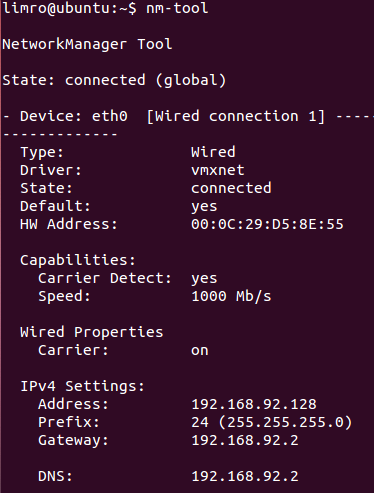
\includegraphics[scale=0.7]{nm-tool.png}
\caption{Use of the command \code{nm-tool}}
\label{fig:nm-tool}
\end{figure}

\begin{figure}[H]
\centering
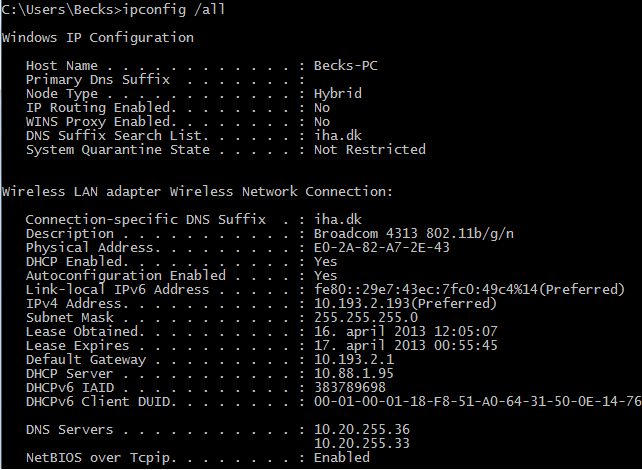
\includegraphics[scale=0.7]{ipconfig.png}
\caption{Use of the command \code{ipconfig /all}}
\label{fig:ipconfig}
\end{figure}

To detect an IP-address and determine the latency to the server use the \code{ping} command.
\code{ping} will target either a webserver name to get the IP-address or target the IP-address directly without asking the DNS-server.
This is shown on figure \ref{fig:ping}


\begin{figure}[H]
\centering
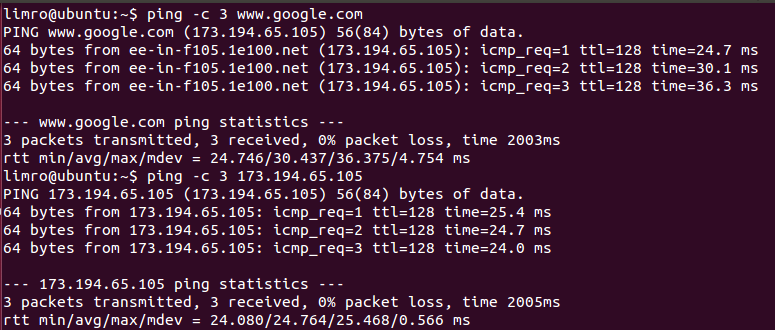
\includegraphics[scale=0.7]{ping}
\caption{Use of the command \code{ping -c 3 www.google.com}}
\label{fig:ping}
\end{figure}


Before making a lookup at the DNS server the system will check local HLT file, located in  \textit{/etc/hosts}, to see if any redirects or A records are listed.
Redirections are created by typing the static IP-address followed by the new logical name as shown in code snippet below.


\begin{lstlisting}[caption={Hosts file redirection}, style=Code-Bash, label=lst:redirect]
# Redirections
212.130.55.139 vejr #Resolve vejr to "www.dmi.dk"
159.20.6.38 nyhed #Resolve nyhed to "www.dr.dk"
157.55.46.241 mail #Resolve mail to "www.hotmail.com"
\end{lstlisting}

\vspace{10px}

When requesting a webserver through a DNS, the root servers first redirect to the top-level domain server, TLD, which contains the '.com', '.net', '.dk' etc \cite[p. 192]{Tanenbaum}.
From here the domain server can return the IP-address for the name server to which the client can connect. 
This will then (most likely) recursively or (less likely) iterative\footnote{See section \ref{sec:nameRes}, Name resolution} return the specified IP-address to the client.
\\
\\
Each DNS server is responsible for looking up domains in nonoverlapping parts called 'zones'. 
A zone is implemented by a separate name server\cite[p. 202-205]{Tanenbaum}.
\\
\\
When looking for a host name there can be multiple units with the same logical name. 
However it is possible to specify a name for a unit to unambiguously unique with a '.' (dot) at the end of the logical address which is called a fully qualified domain name (FQDN)\cite{wiki-fqdn}.
\\
Multiple computers could have the name \textit{myComputer} but if looking for a computer on a network called \textit{work.net.} there can only be one computer with the name \textit{myComputer.work.net.}



\newpage
\section{Name resolution}\label{sec:nameRes}

When looking up an IP-address it can be resolved in two different ways.
In iterative name resolution the root DNS server return the IP-address for the a DNS server which contains information of the requested country code. 
Afterwards the client will ask this DNS server for the IP-address and so on until the client the requested IP-address.
This DNS query/response transaction type of resolution requires the client involvement for each request to a DNS server which leads to lower performance cost for the DNS servers \cite[p. 205-209]{Tanenbaum}.

\begin{figure}[H]
\centering
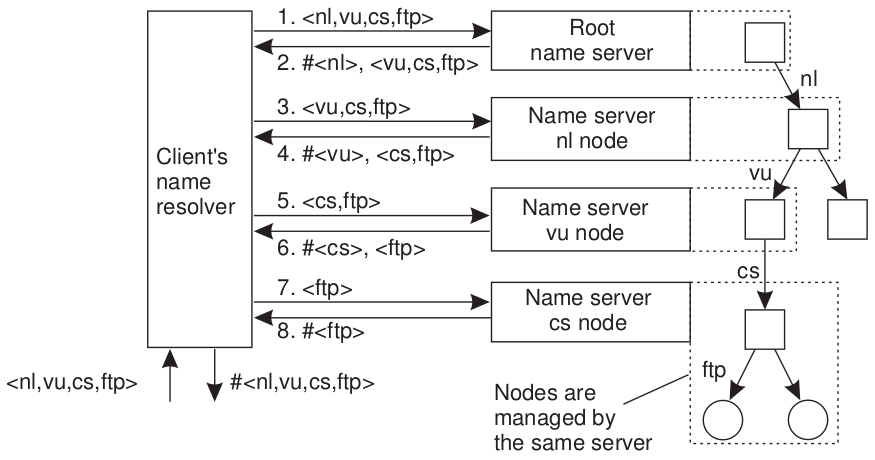
\includegraphics[scale=0.6]{iterativ}
\caption{Iterative request for an IP-address}
\label{fig:iterativ}
\end{figure}


In recursive name resolution the root DNS server will ask the country coded DNS server for the IP-address of the website.
The country coded DNS server ask the another DNS server which contains specific information of the domain and so on, until the website is identified.
The IP-address is returned recursively to the root DNS server and back to the client.
Caching the returned IP-address can lower the performance cost drastically, since a lookup is unnecessary for the same request next time.

Therefore the client is only involved when asking for and obtaining the IP-address which reduce performance cost for the client \cite[p. 205-209]{Tanenbaum}.

\begin{figure}[H]
\centering
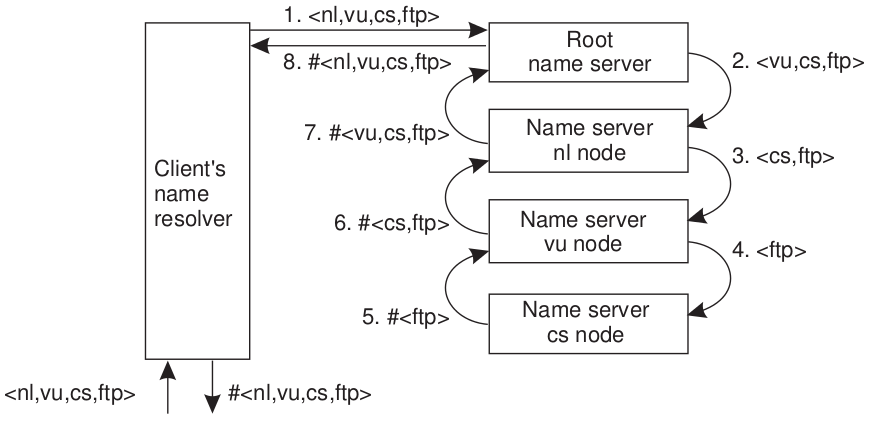
\includegraphics[scale=0.7]{recursiv}
\caption{Iterative request for an IP-address}
\label{fig:recursiv}
\end{figure}


\newpage
\section{DNS security extentions}\label{sec:DNS-security}
Due to security issues various governments, research organizations and others have developed a specification and associated protocol called DNS Security extensions (DNSSEC) which protects DNS querty/response transactions \cite[p. 84]{DNS-article}.

Two main security threats exist for DNS in the context of query/response transactions. Attackers can

	\begin{itemize}%[ref=test]
	\item cheat domain name servers and respond to DNS queries and alter DNS responses

	\item alter the DNS responses stored in caching name servers.
	\item[] \hspace{100mm}\cite[p. 84]{DNS-article}
	\end{itemize} 
DNSSEC was designed to protect the users from obtaining corrupted DNS data. 
It contains a set of extensions to DNS which provide origin authentication of DNS data, authenticated denial of existence, and data integrity. An administrative entity in the domain name system that provides DNS services for a group of domains is called a \textit{zone}.
If a DNS server uses DNSSEC it is marked as a \textit{signed zone} \cite{DNS-article}.



A signed zone is a DNS server zone which includes a digital signature for all content it returns.
It verifies that the underlying responses have requested resource records, special resource records that carry the digital signatures associated with the requested resources and it contains a DNSKey which include a public key which can verify the signature \cite{DNS-article}.



Using signed zones as authentication requires a DNSSEC-aware caching name server which start from a trusted public key stored within it self, a \textit{trust anchor}.
This establish a chain of trusted DNS servers with DNSSEC implemented to the public key of the zone. 
It is also possible to use a \textit{trust anchor list} which contains a list over trusted anchors \cite{DNS-article}.

Currently the boundaries of the secure DNS is at the caching name servers as there is no end-to-end security. It would be preferable if an application could decide weather the requested data was corrupted or not. To accommodate this it it recommended to develop standardized formats or APIs that enabled caching name servers to communicate the security status (information about the outcome of the signature verification) to for example web or mail servers. It could also be met if the web servers performed the signature verification although it could lead to lower performance when small networked devices are used \cite{DNS-article}.



\subsection{Censorship and misuse of DNS}


In 1998 China started the Golden Shield Project because they feared inciting of internet users overthrowing the government, harm national unification, spread rumours e.g.\cite{GFW-avoid} and began, with various techniques, to block the Chinese from websites and searches on the internet.
\\
One of the methods used is by setting up \textit{wiretap} that listens to everything sent out from Chinese internet service providers (ISPs) and DNS resolvers and sending back a fake DNS reply -- a technique called \textit{DNS injection} \cite{GFW}. 


This is one example\footnote{Looking aside from other techniques the Golden Shield provide} where DNSSEC could prove valuable -- reassuring the client the correct IP-address.

\chapter{Prototype: School DNS}
A school want to use a DNS server to filter certain internet sites from students and also have the opportunity to get a faster response from the name server. 

\section{Solution}
To achieve the school's request, a BIND server could be set up. 
BIND is a open source implementation of the DNS protocol and is the most used DNS server software. 
One of the advantages with BIND, is that it supports both Windows, Mac and Linux. 
BIND acts like a caching server, where it stores answers to name queries which results in reduced response time of future queries to the same server.

When a requested hostname needs to be looked up the local cache is the first place to be checked. 
If the hostname is not found there a DNS server is asked. 
This might be your ISP or even a server on a "higher" level. 
It is also possible via BIND to forward your requests to a public DNS server, meaning it will be asked, if no other server before that (e.g. your ISPs DNS server) has the hostname in its cache. An overview of this system is showed in Figure 1.1:

\begin{figure}[H]
\centering
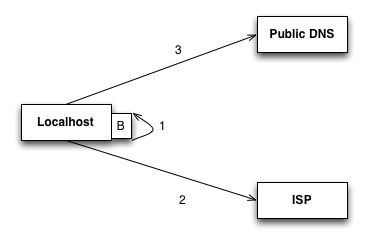
\includegraphics[scale=0.5]{../../Protoypes/DNS/ForwardingDiagram.jpg}
\caption{System overview}
\label{fig:Forwarding}
\end{figure}


\subsection{Setup BIND Server}
To install a BIND server on Linux type in \code{sudo apt-get install bind[9]}. This will install version 9 of the BIND server software. To check if the installation is successful type \code{named -v} where -- if successful, \code{BIND 9.8.1-P1} will be responded. 
For testing purpose, \textit{dnsutils} have been used, because it can be used to see response time for the DNS lookup with the command \code{dig -x [IP-address]}.

\subsection{Caching name server}
A caching name server will find the answer to name queries and remember the answer the next time you need it. To set up the caching name server the configuration file /ect/resolv.conf needs to contain the following:\\ \code{nameserver 127.0.0.1}\\
To test the caching name server type \code{dig ubuntu.com} twice to see that the response time is a lot faster the second time:

\begin{figure}[H]
\begin{minipage}[b]{0.45\linewidth}
\centering
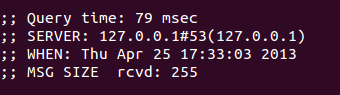
\includegraphics[width=\textwidth]{dig1}
\caption{Use of the command \code{dig ubuntu.com} the first time}
\label{fig:dig1}
\end{minipage}
\hspace{0.5cm}
\begin{minipage}[b]{0.45\linewidth}
\centering
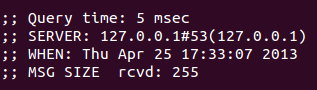
\includegraphics[width=\textwidth]{dig2}
\caption{Use of the command \code{dig ubuntu.com} the second time}
\label{fig:dig2}
\end{minipage}
\end{figure}

\subsection{Forward to public DNS}
If the school wants to forward their requests to a public DNS, e.g. OpenDNS, they have to do a bit of research on finding the optimal solution for them. 
There is a lot of public DNS servers, where some of them are good at filtering bad hostnames, but are in the same time not always the fastest.
In this section tests are made to find the fastest response time.

To find an optimal solution, Google's Test Bench (GTB) have been used.
In this case GTB looked up around 4500 servers and tested them all to find the fastest server in average.

\begin{figure}[H]
\centering
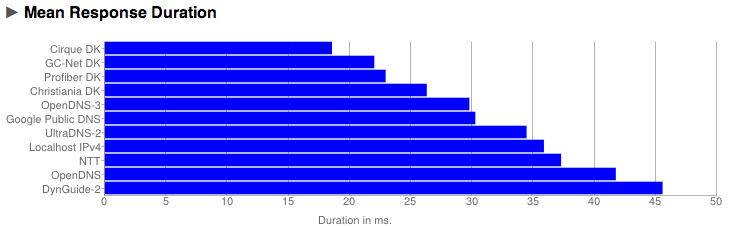
\includegraphics[scale=0.5]{Figurer/NamebenchTest.png}
\caption{Output from Google Test Bench test}
\label{fig:testBench}
\end{figure}

The test in Figure \ref{fig:testBench} and Table \ref{tab:Forwarding} shows, that Cirque DK have the lowest mean response time with 18 ms, and the default DNS have a mean response time on 36 ms. 
One of the more popular public DNS is openDNS, which is a little faster than the default DNS with 29 ms. 

In a way of verifying the results of GTB, a manual test with \code{dig -x} have been made with 5 different internet sites and their given response time. 
To test the servers, the file located at \textit{/etc/bind/named} have to be edited with the address of the DNS server it shall forward to. 

\begin{table}[H]

\begin{center}
  \begin{tabular}{l|c|c}
    \multicolumn{3}{c}{Forwarding - Cirquie.DK}  \\
	\hline Site & First test (ms) & Second test (ms) \\ \hline
    Ubuntu.com & 391 & 381  \\ %\hline
    Bt.dk & 356 & 906  \\ %\hline
	Iha.dk & 375 & 240 \\ %\hline
	Facebook.com & 354 &	207 \\ %\hline
	Wikipedia.org & 375 & 442 \\ \hline
  \end{tabular}
\end{center}
~\\
\begin{center}
  \begin{tabular}{l|c|c}
    \multicolumn{3}{c}{Forwarding - OpenDNS}  \\
	\hline Site & First test (ms) & Second test (ms) \\     
    \hline
    Ubuntu.com & 355 & 352  \\ %\hline
    Bt.dk & 792 & 436  \\ %\hline
	Iha.dk & 334 & 117 \\ %\hline
	Facebook.com & 184 & 279 \\ %\hline
	Wikipedia.org & 153 & 115 \\ \hline
  \end{tabular}
\end{center}
\caption{Forwarding with Cirquie.DK and OpenDNS}
\label{tab:Forwarding}
\end{table}


It is hard to make a final conclusion based on our test, since the response times are unstable (e.g. even though bt.dk was tested via Cirquie.DK two times under the same conditions; first test resulted in 356 ms and second in 906 ms), which is why GTB is a good tool to use. 
However, we can conclude that even if you forward to the one tested to be the fastest public DNS, you cannot be sure it is the fastest every single time, since the server might be busy.

\subsection{Filtering}
A DNS server can also be used as a simple filter, in the way of not providing the IP for harmful or illegal hostnames. 
Some public DNS servers, like OpenDNS, have this filter build-in, which means that you in a simple way can archive a bit of security.

In the same way, it is also possible to block specific hostnames with BIND, which can be useful if you want your filter to be more specialized. 
This can be used if a school wants to block for e.g. Facebook or Ekstrabladet.dk.

The problem about this way of filtering is if the users look up the IP directly. 
In that case, the DNS server will not be used and the filter will therefore not be used either and other methods have to be used.

\chapter{Conclusion}

\section{Conclusion}
%Conlude on your investigations.

The DNS system is a cleaver solution to the original problem; connecting millions of computers through the internet.
In many aspects the system is brilliant resolving human friendly logical names into IP address meanwhile being very fast and does not need user interference. Although there is no assurance that the requested data is not corrupted as the name servers can be cheated with altered DNS responses as outcome. Currently it can be guaranteed that DNS query/response transactions is secure if the digital signature-based DNSSEC is being used. Unfortunately the DNSSEC does not cover mail servers, web browsers or web servers.
\\
\\
There is a lot of ways of finding a solution for the school used as case in the prototype-development.
To retrieve the caching functionality, BIND is simple and easy to set up and use. 
If wanted, it can furthermore be specialized in the way of setting up a filter or forwarding requests to a public DNS server.  
\\
BIND is a simple solution, but if better security or caching is wanted, a custom solution is needed. However, for a small school this might not be needed, and therefore BIND would be the suggested choice.


\section{Discussion}
% Discuss your project work.

The internet is a great system used by millions of computers every day and DNS servers are one of the main factors for its accessibility. 
Due to this fact it is necessary that no politic organization can shut down the servers to prevent the citizens access to the internet.
\\
\\
Security measures has been taken but a country like China has found loopholes to censor part of the internet, setting up \textit{Deep Packet Inspection} near all international gateways and searching for certain keyword, they  return bad IP-addresses before the correct is returned\cite{GFW}.\\
If it was "only" China's population who could not access certain websites it would be a relatively controlled problem, but if a computer in South Korea request a website and the location of the root DNS server is in China, South Korea is suddenly also affected.
\\
\\
Also it is significant that the security of the DNS query/response transaction is limited to the caching name servers as it can not be guaranteed that a web server is not attacked. Also the DNSSEC developers can not require implementation of the DNSSEC. As a result the users have to rely on their ISPs filters or they can use BIND with customized filtering.


%\nocite{*}
\bibliographystyle{ieeetr}
\bibliography{references}

%\end{thebibliography}

\end{document}